Import kan som tidigare nämts ske till och från .xml-filer. Dessa kan
med fördel skrivas för hand och importeras ifall man föredrar att mata
in sina recept med tangentbordet istället. Är användaren bekant med
xml finns en exempelfil att se i fig \ref{fig:xml}. Här följer en kort
beskrivning av formatet.

I xml används taggar på formen \verb+<tag>+ Någon form av inmatning \verb+</tag>+

De taggar som används i matlabb är
\begin{itemize}
\item \verb+<recipe>+ Anger receptnamn
\item \verb+<portionsize>+ Anger portionsstorlek på receptet
\item \verb+<ingredient>+ Anger ingredienser (sedan tidigare tillagd i
  databasen)
\item \verb+<amount>+ Anger mängd av ingrediensen
\item \verb+<unit>+ Anger en enhet till antalet
\item \verb+<instruction>+ Anger instruktioner till receptet
\item \verb+<time>+ Anger tid
\item \verb+<price>+ Anger pris (frivillig)
\item \verb+<energy>+ Anger engeriinnehåll (frivillig)
\item \verb+<rating>+ Anger betyg.

Taggarna hänger ihop genom att \verb+<recipe>+ omsluter hela
receptet. \verb+<ingredient>+ omsluter \verb+<amount>+ som i sin tur
omsluter \verb+unit+.

Vill man lägga till fler ingredienser än en är det bara att lägga till
fler \verb+<ingredient>+ taggar. I \ref{fig:xml} finns ett klargörande exempel.
 
\end{itemize}



\begin{figure}[H]
         
        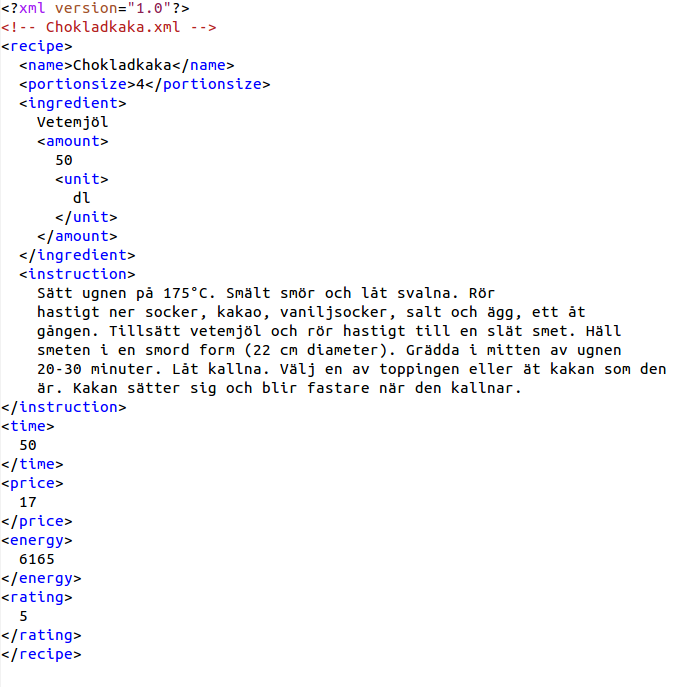
\includegraphics[scale=0.44]{xml.png} 
        \caption{Exempel xml-fil} 
        \label{fig:xml}
\end{figure} 
